Firstly, we will explain the metric system of the evaluation Dataset that the researchers who wanted to evaluate the AlphaPose as well as many other models used. More specifically, the evaluation dataset which we are going to discuss is the MS COCO \cite{MS COCO} (Microsoft Common Objects in Context) which is a large-scale object detection, segmentation, key-point detection, and captioning dataset. The dataset consists of 328K images. It contains 164K images split into training (83K), validation (41K) and test (41K) sets. Therefore, as we mentioned this Dataset can be used to evaluate both object detection and key-point detection. Subsequently, we can evaluate the AlphaPose model which contains two different models, the Yolo model for the object detection and the keypoints Detection using the SPPE model.\\

To evaluate these algorithms, the metric system that we will use is the AP \cite{AP} (Average Precision) and mAP (Mean Average Precision). Let's start with the definition of precision and recall. 
$$ Precision = \dfrac{tp}{tp+fp}$$
$$ Recall = \dfrac{tp}{tp+fn}$$
where, tp = true positive, fp = false positive, fn = false negative. \\

In order to verify a result as tp, fp, or fn, there are put some thresholds. For example, in object detection where we want to classify an object as well as we need to put it inside a box, we compare the label that we classified, and about the box, we check the Intersection over the union (IoU) of the true box location and the estimated box location. Sometimes the IoU threshold is fixed, for example, at 50\% or 75\%, which are called AP50 and AP75, respectively.\\

So basically precision is measuring the percentage of correct positive predictions among all predictions made, and recall is measuring the percentage of correct positive predictions among all positive cases in reality. There is always a trade-off between the two metrics. Imagine if we label everything as positive, then recall will be 1 because we do not have false negatives, but precision will be horrible because only a small percentage of our positive predictions are actually correct. In the other extreme case, we can be very careful about the selection of positive prediction, so prediction will be very good, but we might have labeled many positive cases as negative and consequently lowered recall. Generally, Recall values increase as we go down the prediction ranking. However, precision has a zigzag pattern, where it goes down with false positives and goes up again with true positives. In the figure below we display this Graph pattern.\\

\begin{figure}[htp]
    \centering
    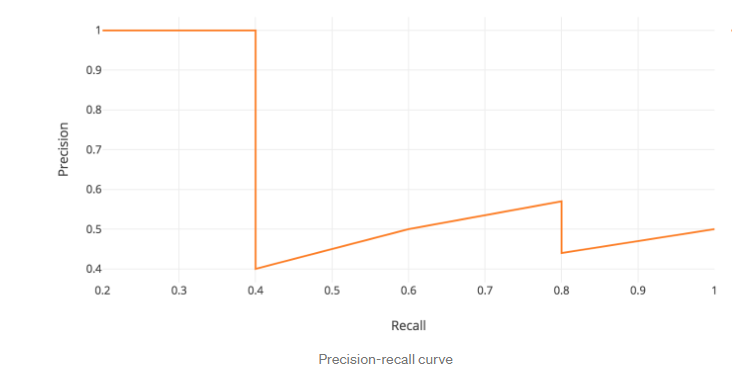
\includegraphics[width=7cm]{figures/Evaluation/AP1.png}%
    \qquad
    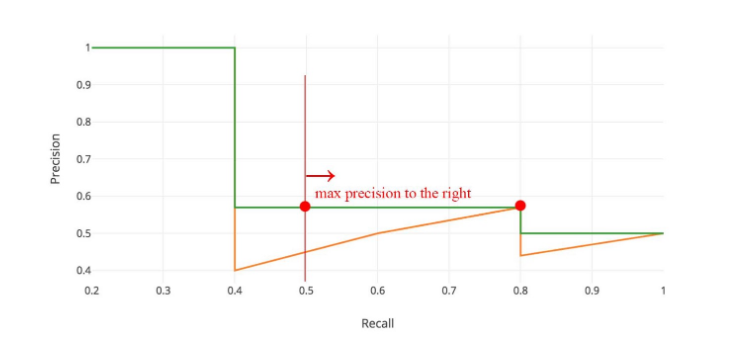
\includegraphics[width=7cm]{figures/Evaluation/AP2.png}%
    \captionsetup{labelformat=empty}
	\caption{\href{https://jonathan-hui.medium.com/map-mean-average-precision-for-object-detection-45c121a31173}
	{Example of normal and a smoothed Precision-recall curve}}
\end{figure}


The general definition for the Average Precision (AP) is finding the area under the precision-recall curve above. Precision and recall are always between 0 and 1. Therefore, AP falls within 0 and 1 also. Before calculating AP for the object detection, we often smooth out the above graph pattern first. Therefore, the AP can be calculated from the smoothed Precision-recall curve as:

$$ AP = \int^1_0 p(r)dr $$
where p(r) is the Precision-recall curve graph.\\

At this point, we are ready to display the results of the AlphaPose evaluation with this metric system.
Firstly, the Yolo model which we used compared to many other similar models, the AP in MS COCO Dataset is shown in the figure below : 

\begin{figure}[htp]
	\centering
	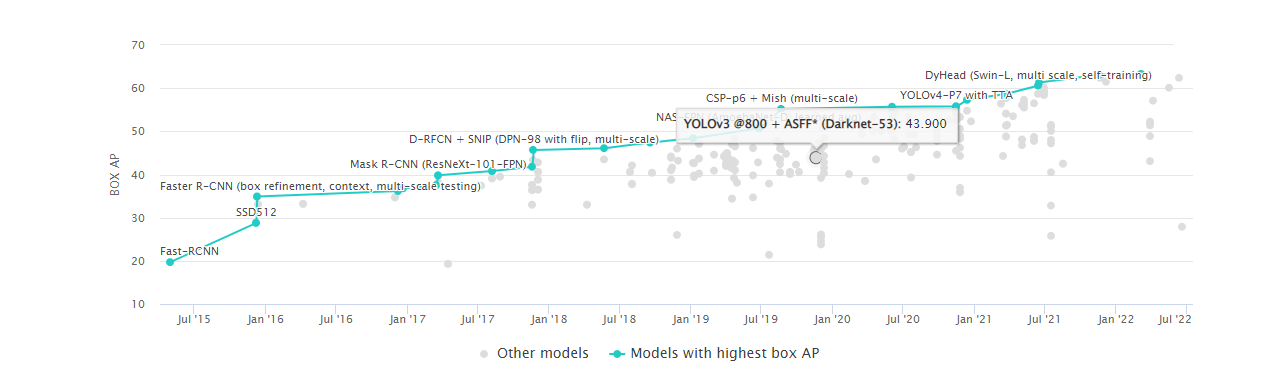
\includegraphics[width=1\textwidth]{figures/Evaluation/YoloEvaluation.png}
	\captionsetup{labelformat=empty}
    \caption{\href{https://paperswithcode.com/sota/object-detection-on-coco}
	{Yolov3 model box Average Precision evaluation compared to other model}}
	\hspace{1em}%
	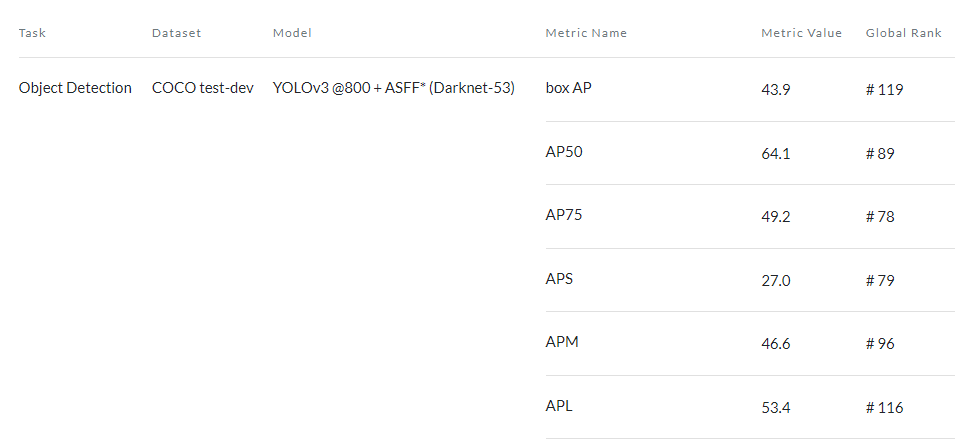
\includegraphics[width=1\textwidth]{figures/Evaluation/TotalEvalutationYolo.png}
	\captionsetup{labelformat=empty}
	\caption{\href{https://paperswithcode.com/paper/learning-spatial-fusion-for-single-shot}
	{Yolov3 Object Detection results on the MS COCO test-dev dataset of some typical baselines. AP, AP50 , AP75 scores (\%). APS:AP of small objects, APM:AP of medium objects, APL:AP of large objects.}}
\end{figure}

Regarding the SPPE model, again with the same Dataset as well as the OCHuman Dataset \cite{OCHuman}. OCHuman is focused on heavily occluded humans. It contains 4731 images and 8110 persons labeled with 17 keypoints. In OCHuman, on an average 67\% of the bounding box area has overlap with other bounding
boxes, compared to only 0.8\% for COCO. Additionally, the number of examples with occlusion IoU > 0.5 is68\% for OCHuman, compared to 1\% for COCO. This makes the OCHuman dataset complex and challenging for human pose estimation. In the figure below, we present the evaluation results for these Dataset, for the AP metric system, as well as the comparison of AlphaPose SPPE model to similar models.

\pagebreak

\begin{figure}[h]
	\centering
	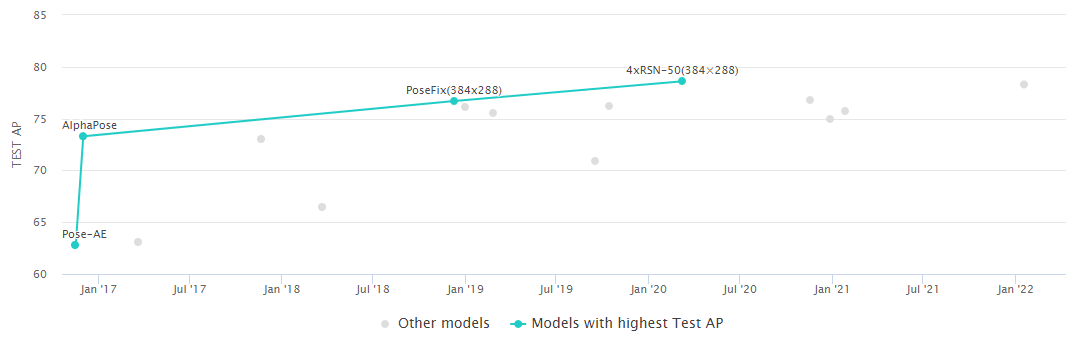
\includegraphics[width=0.8\textwidth]{figures/Evaluation/SPEEComparison.png}
	\captionsetup{labelformat=empty}
	\caption{\href{https://paperswithcode.com/sota/keypoint-detection-on-coco}
	{AlphaPose SPPE model Average Precision tests evaluation compared to other keypoint Detection Models}}
\end{figure}

\begin{figure}[h]
	\centering
	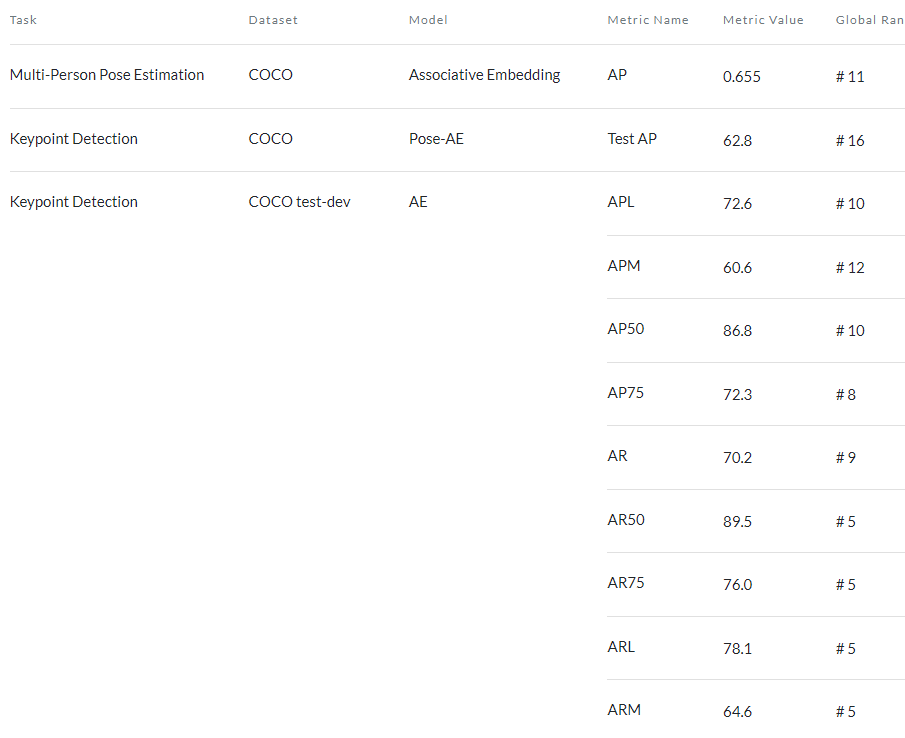
\includegraphics[width=0.7\textwidth]{figures/Evaluation/EvaluationSPEE1.png}
	\captionsetup{labelformat=empty}
	\caption{\href{https://paperswithcode.com/paper/associative-embedding-end-to-end-learning-for}
	{SPPE model Average Precision tests evaluation on COCO Dataset}}
\end{figure}

\pagebreak

\begin{figure}[h]
	\centering
	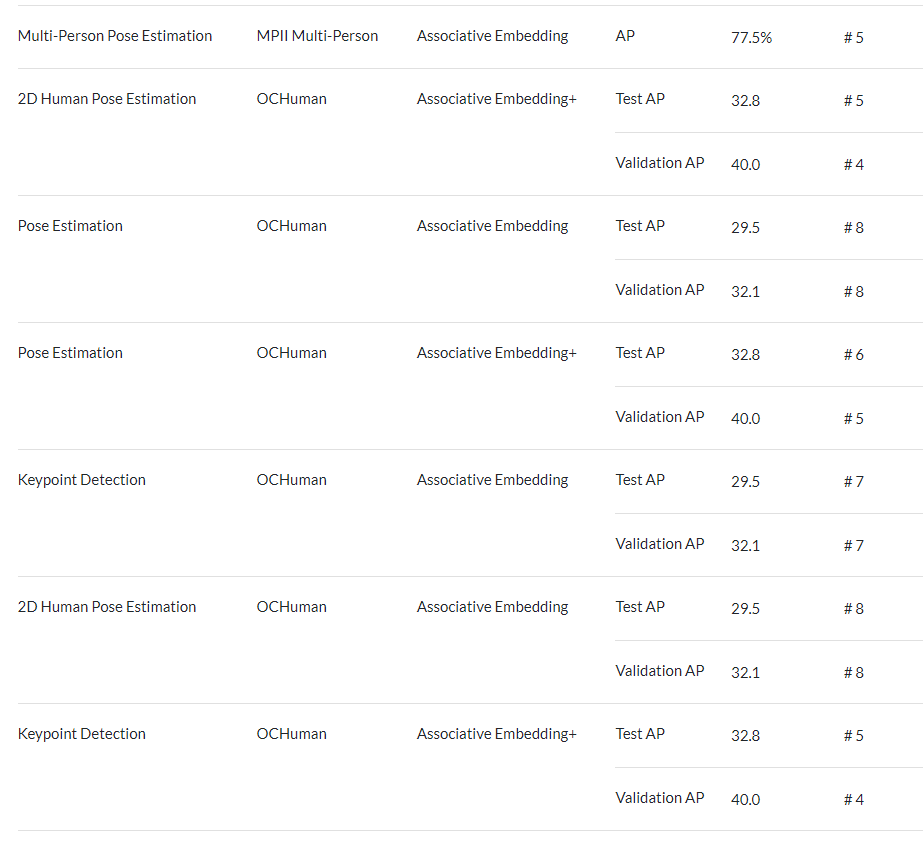
\includegraphics[width=0.7\textwidth]{figures/Evaluation/EvaluationSPEE2.png}
	\captionsetup{labelformat=empty}
	\caption{\href{https://paperswithcode.com/paper/associative-embedding-end-to-end-learning-for}
	{SPPE model Average Precision tests evaluation on OCHuman Dataset.}}
\end{figure}


